% !TeX program = lualatex
% Copyright 2004 by Till Tantau <tantau@users.sourceforge.net>.
%
% In principle, this file can be redistributed and/or modified under
% the terms of the GNU Public License, version 2.
%
% However, this file is supposed to be a template to be modified
% for your own needs. For this reason, if you use this file as a
% template and not specifically distribute it as part of a another
% package/program, I grant the extra permission to freely copy and
% modify this file as you see fit and even to delete this copyright
% notice. 

\documentclass{beamer}
\usepackage[utf8]{inputenc}
\usepackage{physics}
\usepackage[english]{babel}
\usepackage{graphicx}
\usepackage{tikz}
\usepackage{multicol}
\usepackage{subfig}
\usepackage[backend=biber,natbib, maxcitenames=1,style=apa]{biblatex}
\DeclareLanguageMapping{english}{english-apa}
\addbibresource{refs.bib} 
\usetheme{CambridgeUS} %Roja nice
% ---- Itemize Specifier ----
\setbeamertemplate{itemize items}[square]
\setbeamertemplate{enumerate items}[square]
% Table of contents size subsections and subsubsections
\setbeamerfont{subsection in toc}{size=\scriptsize}
\setbeamerfont{subsubsection in toc}{size=\scriptsize}

% Table of contents (Enumeration shapes)
\setbeamertemplate{section in toc}[square]
\setbeamertemplate{subsection in toc}[square]
\setbeamertemplate{subsubsection in toc}[square]
\setbeamercovered{transparent} 
% Colors
\definecolor{swissred}{rgb}{0.93, 0, 0}%{0.93, 0.19, 0.10}
\setbeamercolor*{footer color1}{fg=white,bg=swissred} % dark red
\setbeamercolor{palette tertiary}{fg=white, bg=swissred}
\setbeamercolor{palette primary}{fg=black}
\setbeamercolor{palette secondary}{fg=black}
\setbeamercolor{frametitle}{fg=swissred}
\setbeamercolor{title}{fg=swissred}
\setbeamercolor{itemize item}{fg=red}
\setbeamercolor{itemize subitem}{fg=red}
\setbeamercolor{enumerate number projected}{bg=red}
\setbeamercolor{section number projected}{bg=red,fg=white}
\setbeamercolor{subsection number projected}{bg=red,fg=white}
\setbeamercolor{subsubsection number projected}{bg=red,fg=white}

\usepackage[alsoload=astro]{siunitx}
\DeclareSIUnit\h{\mathnormal{h}}
\sisetup{separate-uncertainty = true,
	bracket-numbers=true}

\usepackage[font=small, justification=centering]{caption}
\DeclareCaptionFont{tiny}{\footnotesize}
\captionsetup{font=tiny}
\captionsetup[figure]{labelformat=empty}% redefines the caption setup of the figures environment in the beamer class.
\captionsetup[sub]{font=tiny,labelfont=tiny}
\title[Effects of systematics on void BAO]{Analysis of the response of void BAO to systematic effects in the SDSS observations using mock datasets}

% A subtitle is optional and this may be deleted


\author{Daniel Forero-S\'anchez\inst{\dag}}
% - Give the names in the same order as the appear in the paper.
% - Use the \inst{?} command only if the authors have different
%   affiliation.

\institute[EPFL] % (optional, but mostly needed)
{
  \inst{\dag}%
  Laboratory of Astrophysics (LASTRO)\\
  \vspace{5mm}
  École Polytechnyque Fédérale de Lausanne (EPFL)\\
  Lausanne, Suisse
  
  }
% - Use the \inst command only if there are several affiliations.
% - Keep it simple, no one is interested in your street address.

\date{\today}
% - Either use conference name or its abbreviation.
% - Not really informative to the audience, more for people (including
%   yourself) who are reading the slides online

%\subject{Theoretical Computer Science}
% This is only inserted into the PDF information catalog. Can be left
% out. 

% If you have a file called "university-logo-filename.xxx", where xxx
% is a graphic format that can be processed by latex or pdflatex,
% resp., then you can add a logo as follows:
 \pgfdeclareimage[height=0.7cm]{university-logo}{EPFL_Logo_Digital_RGB_PROD.png}
 \logo{\pgfuseimage{university-logo}}

% \pgfdeclareimage[height=0.5cm]{university-logo}{university-logo-filename}
% \logo{\pgfuseimage{university-logo}}

% Delete this, if you do not want the table of contents to pop up at
% the beginning of each subsection:
\iffalse
\AtBeginSubsection[]
{
  \begin{frame}<beamer>{Outline}
    \tableofcontents[currentsection,currentsubsection]
  \end{frame}
}
\fi
\usepackage{amsmath}
% Let's get started
\begin{document}

\begin{frame}
  \titlepage
\end{frame}

\begin{frame}[allowframebreaks]{Outline}
	\begin{multicols}{2}
		\tableofcontents
	\end{multicols}

  % You might wish to add the option [pausesections]
\end{frame}
\section{Introduction}


\begin{frame}[allowframebreaks]{Introduction}

				\begin{itemize}
					\item The use of voids + matter ones $\Rightarrow$ $\sim10\%$ improvement of error \& 20\% survey size increase.
					\item Voids could be less sensitive to systematic effects than matter.
					\item We want to use mocks to check if there is a difference in the BAO peak shift due to systematical effects between matter tracers and voids.
					\item Systematics can greatly affect the measurement of the 2PCF in real data
				\end{itemize}

\end{frame}
\section{Voids}
\begin{frame}[allowframebreaks]{Voids}
	Definition is controversial, we use a \textbf{geometrical} one.\\
	Delaunay Triangulation $\longrightarrow$ Voids are circumspheres in the simplices with tracers as vertices.\\
	\vspace{1cm}
	\begin{columns}
		\begin{column}{0.45\linewidth}
			\textbf{Small voids}
			\begin{itemize}
				\item Radius cut: $R_c < \SI{8}{\h^{-1} \mega\parsec}$
				\item Located in regions with high $\delta_{dm}$
				\item Correlated with galaxy sample
				\item Are actually Dark Matter
			\end{itemize}
		\end{column}
		\begin{column}{0.45\linewidth}
			\textbf{Big voids}
			\begin{itemize}
				\item Radius cut: $R_c > \SI{15.5}{\h^{-1} \mega\parsec}$
				\item Located in regions with low $\delta_{dm}$
				\item Anticorrelated with galaxy sample
				\item Are actually empty
			\end{itemize}
		\end{column}
	\end{columns}
\pagebreak
\begin{columns}
	\begin{column}{0.49\linewidth}
		\begin{figure}
			\centering
			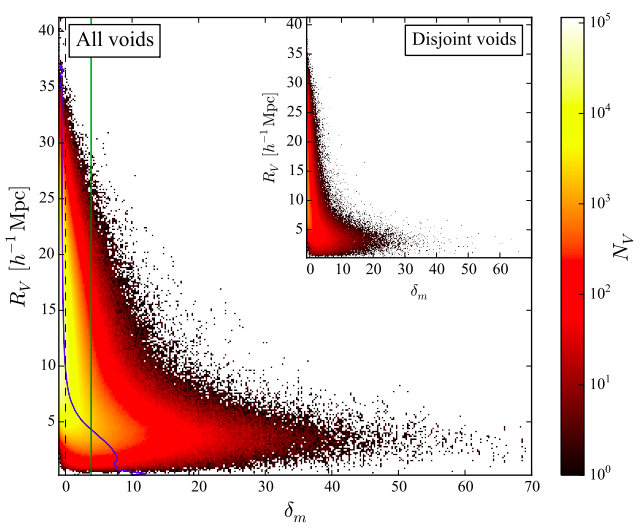
\includegraphics[width=1\linewidth]{plots/radiusvsdensity}
			\caption{Number of voids, $N_V$, as a function of Dark Matter density, $\delta_{dm}$, and void radius, $R_V$. Taken from \citep{Zhao2016}}
			\label{fig:radiusvsdensity}
		\end{figure}
	\end{column}
	\begin{column}{0.49\linewidth}
		\textbf{How do we know?}
		\begin{itemize}
			\item Large voids are constrained to regions with low matter density.
			\item Small void population spans a wide range of densities.
		\end{itemize}
	
	\end{column}
\end{columns}
\end{frame}
\section{Data}
\begin{frame}[allowframebreaks]{Data}
	We use 1000 \textbf{EZ mocks} \citet{Zhao2020}.
	\begin{itemize}
		\item Displacement field from Zel'dovich
		\item PDF extraction from n-body simulation
		\item Halo position assignment
	\end{itemize}
\begin{table}
	\centering
	\caption{Fiducial cosmology parameters used to produce the EZmocks used in this work.}
	\label{tab:fiducial}
	\begin{tabular}{cc}
		\hline
		Parameter & Value \\
		\hline
		$\Omega_m$ & 0.307115 \\
		$\Omega_b$ & 0.048206\\
		$h$ & 0.6777 \\
		$\sigma_8$ & 0.8225\\
		$n_s$ & 0.9611\\
		\hline
	\end{tabular}	
\end{table}
\end{frame}
\section{Systematics}
\begin{frame}[allowframebreaks]{Systematics: Fiber collisions}
	\begin{itemize}
		\item Objects too close in the sky ($r_{cp}<62''$) can't be seen at the same time due o width of the fiber.
		\item One is measured by the plate. The other one(s) could still be measured by other plate.
		\item Define $\mathrm{TSR} = \frac{\mathrm{measured\ targets}}{\mathrm{total\ number\ of\ targets}},$ per sector.
		\item Compensate this effect with $w_{cp} \approx \mathrm{TSR}^{-1}$\\ Actually $w_{cp} = \frac{\mathrm{total\ number\ of\ targets}}{\mathrm{measured\ targets}}$ but defined per \textbf{collision group}.
	\end{itemize}
\end{frame}
\begin{frame}[allowframebreaks]{Systematics: Redshift Failures}
	\begin{itemize}
		\item Errors in the spectroscopic pipeline $\Rightarrow\ \mathrm{SSR}<1$. 
		\item Two sources of error: Observational conditions \& Position of fiber
		\item This is corrected by the weight
		$$w_{noz}\equiv \qty(\mathrm{SSR}_{\mathrm{obs}}\mathrm{SSR}_{\mathrm{pos}})^{-1}.$$
	\end{itemize}
\end{frame}
\begin{frame}[allowframebreaks]{Systematics: Angular Photometric}
	\begin{itemize}
		\item Represented as \textsc{Healpix} maps containing different photometric parameters, $p_i$.
			\item Parameters are combined as $$y^k = \epsilon + \sum_i c_ip_i^k$$ where the model weights, $c_i$ are optimized (per chunk) such that $n_{\mathrm{dat},k} \approx n_{\mathrm{ran},k}y^k$, where $k$ indicates the pixels.
			%$$c_i = \arg\min_{c_j}\sum_{k\in\mathrm{chunk}}\frac{n_{\mathrm{dat},k} - n_{\mathrm{ran},k}y^k(c_j)}{\sqrt{n_{\mathrm{ran}, k}}}$$
		\item The photometric weights designed to partially correct for these effects are defined as $$w_{\mathrm{systot}} = \qty(y^k)^{-1}.$$
	\end{itemize}
\end{frame}
\begin{frame}[allowframebreaks]{Systematics: Normalization}
\begin{itemize}
	\item Completeness weights are defined as:
	$$w_{\mathrm{comp}} = w_{\mathrm{systot}}w_{cp}w_{noz}.$$
	\item Some normalization is done (on $w_{\mathrm{systot}}$ before $w_{\mathrm{comp}}$ and on $w_{noz}$ after).
	\item Invalid objects are set $w_{cp}, w_{noz} = 0$.
	\item Only elements with $\mathrm{SSR}\geq0$, $z\in(0.6, 1.1)$ and completeness $> 50\%$ are selected.
	\item The dependence on $n(z)$ is corrected by $$w_{\mathrm{FKP}} \equiv \frac{1}{1 + n(z) P_0};\quad P_0 = \SI{4000}{\h^{-3}\mega\parsec\cubic}.$$
\end{itemize}
\end{frame}

\begin{frame}[allowframebreaks]{Systematics: Application}
	\begin{itemize}
		\item We compute $w_{\mathrm{comp}}^{\textsc{allsyst}} =w_{\mathrm{systot}}w_{cp}w_{noz}w_{\mathrm{FKP}}$ and the effective number of tracers in each chunk $$n_{eff} = \sum_{i=1}^{N_{chunk}}w_{\mathrm{comp},i}^{\textsc{allsyst}},$$ where $N_{chunk}$ is the number of tracers in the chunk considered.
		\item We then compute $$w_{\mathrm{comp}}^{\textsc{partial}}=w_{\mathrm{FKP}}\prod_{s\in \mathcal{S}'}w_s,$$ where $\mathcal{S}' \subseteq \mathcal{S}$ is the subset of systematic effects to be considered and $\mathcal{S} =\qty{\mathrm{systot},\ noz,\ cp}$. In this case we compute the new effective number of tracers $$n'_{eff} = \sum_{i=1}^{N_{chunk}}w_{\mathrm{comp},i}^{\textsc{partial}}.$$
		\item Objects in the catalog with $w_{\mathrm{comp}}^{\textsc{partial}}=0$ or $\mathtt{veto}=0$ (such as objects outside the survey area or masked by bright stars) are removed.
		\item We then normalize the completeness weights in each chunk by the corresponding $n_{eff}/n'_{eff}$ to keep the original effective number of tracers.
	\end{itemize}
\end{frame}
\section{Catalog generation}
\begin{frame}[allowframebreaks]{Catalog generation}

	\begin{itemize}
	\item Export catalogs with $$\mathrm{RA},\ \mathrm{DEC},\ z,\ w_{cp}w_{\mathrm{FKP}},\ w_{cp},\ w_{\mathrm{FKP}},\ n(z)$$
	\item Use \textsc{Dive} to extract void catalogs with (we use $\Omega_m=0.31$)
	$$\mathrm{RA},\ \mathrm{DEC},\ z,\ R$$
	\begin{multicols}{2}
	\item Mask void catalogs
	\item Create void randoms
	\small
	\begin{itemize}
		\item Combine 100 void mocks
		\item Divide into $z$ bins
		\item divide each bin in $R$ bins
		\item Split ``vertically'' into $\mathrm{RA},\ \mathrm{DEC}\ |\ z,\ R$.
		\item Shuffle one of the two halves.
		\item Recombine halves and all bins.
		\item Randomly choose $\num{2700000}$ with $R>R_c(=\SI{15.5}{\h^{-1}\mega\parsec})$
	\end{itemize}
	\normalsize
	\end{multicols}
\end{itemize}



\end{frame}
\section{Radius cut}
\begin{frame}[allowframebreaks]{Radius cut}
	\begin{columns}
		\begin{column}{0.49\linewidth}
	Analyze signal-to-noise ratio ($\mathrm{SNR}\equiv\frac{\langle S \rangle}{\sigma_S}$) for 100 void mocks with different $R_c$. Use definition of signal, $S$, as in \citet{Liang2016}.
\begin{equation}
\begin{split}
&S = \xi_0(s^{\mathrm{BAO}}) -\\ 
&\frac{\xi_0(s_1^{\mathrm{dl}}) + \xi_0(s_2^{\mathrm{dl}}) + \xi_0(s_1^{\mathrm{dr}}) +  \xi_0(s_2^{\mathrm{dr}})}{4}
\end{split}
\end{equation}
		\end{column}

\begin{column}{0.49\linewidth}
	\begin{figure}
	\centering
	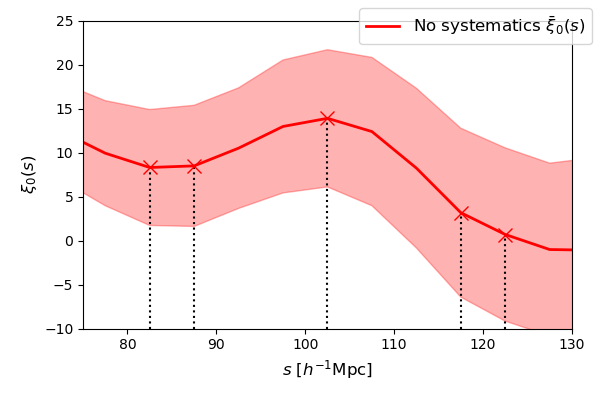
\includegraphics[width=\linewidth]{plots/snr_points}
	\caption{$s_1^{\mathrm{dl}} = 82.5$, $s_2^{\mathrm{dl}}=87.5$, $s_1^{\mathrm{BAO}} = 102.5$, $s_1^{\mathrm{dr}} = 117.5$ and $s_2^{\mathrm{dr}}=\SI{122.5}{\h^{-1}\mega\parsec}$ respectively from left to right.}
	\label{fig:snrpoints}
\end{figure}
\end{column}
\end{columns}
\pagebreak
\begin{figure}
	\centering
	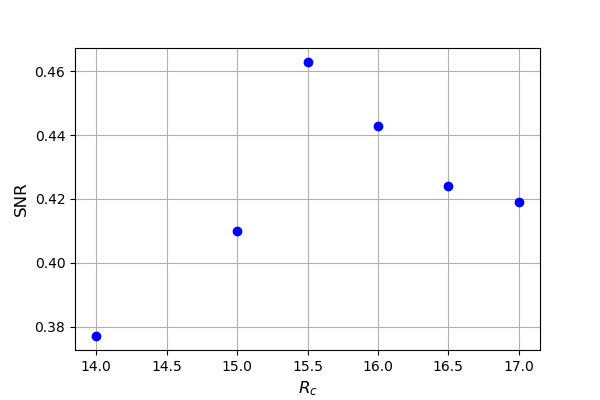
\includegraphics[width=0.5\linewidth]{plots/snr}
	\caption{SNR vs low radius cut $R_c$. Upper cut is always set to $\SI{50}{\h^{-1}\mega\parsec}$. Maximum SNR is obtained for $R_c = \SI{15.5}{\h^{-1}\mega\parsec}$.}
	\label{fig:snr}
\end{figure}
\end{frame}
\section{Model}
\begin{frame}[allowframebreaks]{The BAO model}
	We use the model in \citet{Zhao2019}:
	\begin{align}
&	\xi_t(s) = \int\frac{k^2\dd k}{2\pi^2}\frac{\sin ks}{ks}P_t(k)\exp(-k^2a^2),\quad a = \SI{1}{\h^{-1}\mega\parsec}\\
&	P_t(k) = \qty{\qty[P_{\mathrm{lin}}(k) - P_{\mathrm{nw}}(k)]\exp\qty(\frac{-\Sigma_{\mathrm{nl}}^2k^2}{2}) + P_{\mathrm{nw}}(k)}\frac{P_{\mathrm{t,nw}}(k)}{P_{\mathrm{lin,nw}}(k)},\\
&	\xi_{\mathrm{model}}(s) \equiv B^2 \xi_t(\alpha s) + A(s),\quad A(s) = \frac{a_1}{s^2} + \frac{a_2}{s} + a_3
	\label{eq:pktmod}
	\end{align}
	\begin{table}
		\begin{tabular}{lc|c}
			&Galaxies & Voids\\
			$\frac{P_{\mathrm{t,nw}}(k)}{P_{\mathrm{lin,nw}}(k)}$&1 & $1+ck^2$
		\end{tabular}
	\end{table}
\end{frame}
\begin{frame}[allowframebreaks]{Parameter fitting}
\begin{columns}
	\begin{column}{0.49\linewidth}
		Bayesian inference for parameter $\Theta$: 
		\begin{equation}
		\begin{split}
		p(\Theta|X) &= \frac{p(X|\Theta)p(\Theta)}{p(X)} \\&= \frac{\mathcal{L}(X|\Theta)p(\Theta)}{\mathcal{Z}},
		\end{split}
		\label{eq:bayes}
		\end{equation}
	\end{column}
	\begin{column}{0.49\linewidth}
		\begin{figure}
			\centering
			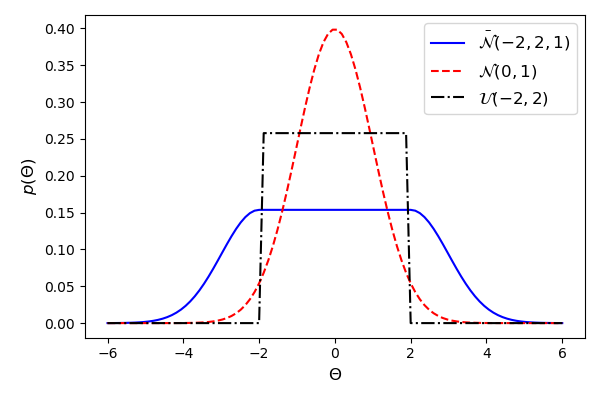
\includegraphics[width=1\linewidth]{plots/priors}
			\caption{Examples of the different kinds of priors used in the fitting.}
			\label{fig:priors}
		\end{figure}

	\end{column}
\end{columns}
\pagebreak
\begin{columns}
	\begin{column}{0.49\linewidth}
		\textbf{Voids}
		\begin{align}
		&p(\Sigma_{\mathrm{nl}}) = \mathcal{U}(0, 20)\\
		&p(B) = \mathcal{N}(2, 0.15)\\
		&p(\alpha)=\mathcal{U}(0.8, 0.12)\\
		&p(c) = \bar{\mathcal{N}}(-500, 1000, 100)
		\end{align}
	\end{column}
	\begin{column}{0.49\linewidth}
		\textbf{Galaxies}
		\begin{align}
		&p(\Sigma_{\mathrm{nl}}) = \mathcal{U}(5, 17)\\
		&p(B) = \bar{\mathcal{N}}(1.4, 1.6, 0.12)\\
		&p(\alpha)=\mathcal{U}(0.8, 0.12)
		\end{align}
	\end{column}
\end{columns}
\end{frame}
\begin{frame}[allowframebreaks]{Results: Mean 2PCF Galaxies}
\begin{multicols}{2}
\textbf{No systematics}
\begin{figure}
	\centering
	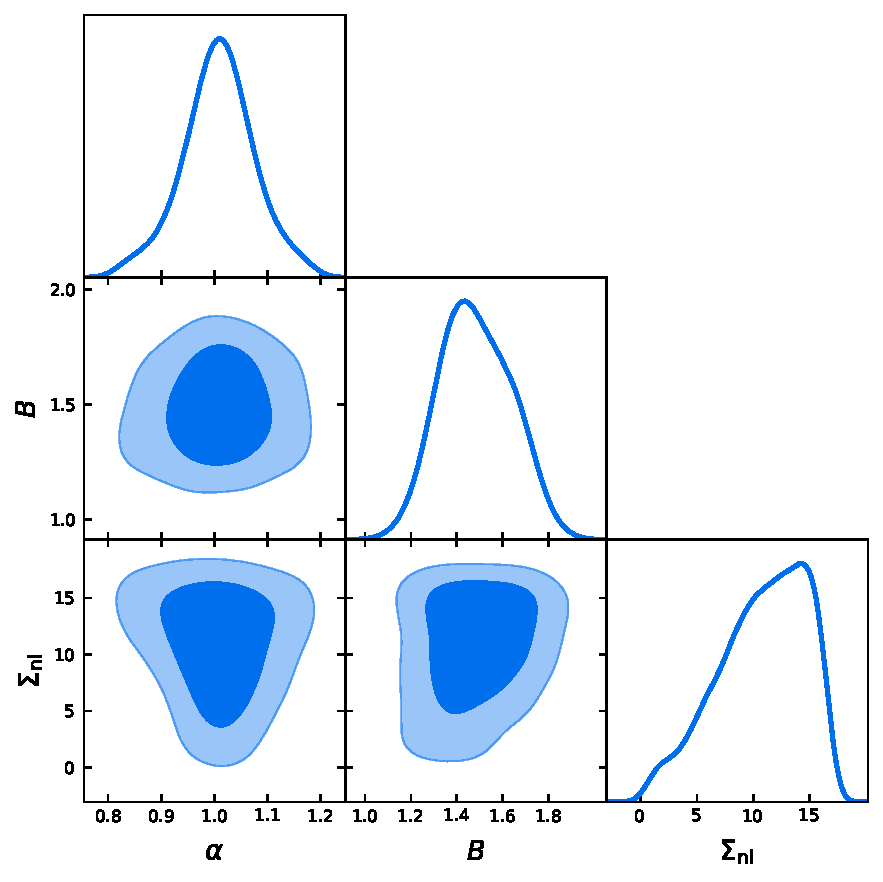
\includegraphics[width=0.9\linewidth]{plots/TwoPCF_mockavg_nosyst_v7_gal_cbz_triplot}
\end{figure}
\textbf{All systematics}
\begin{figure}
	\centering
	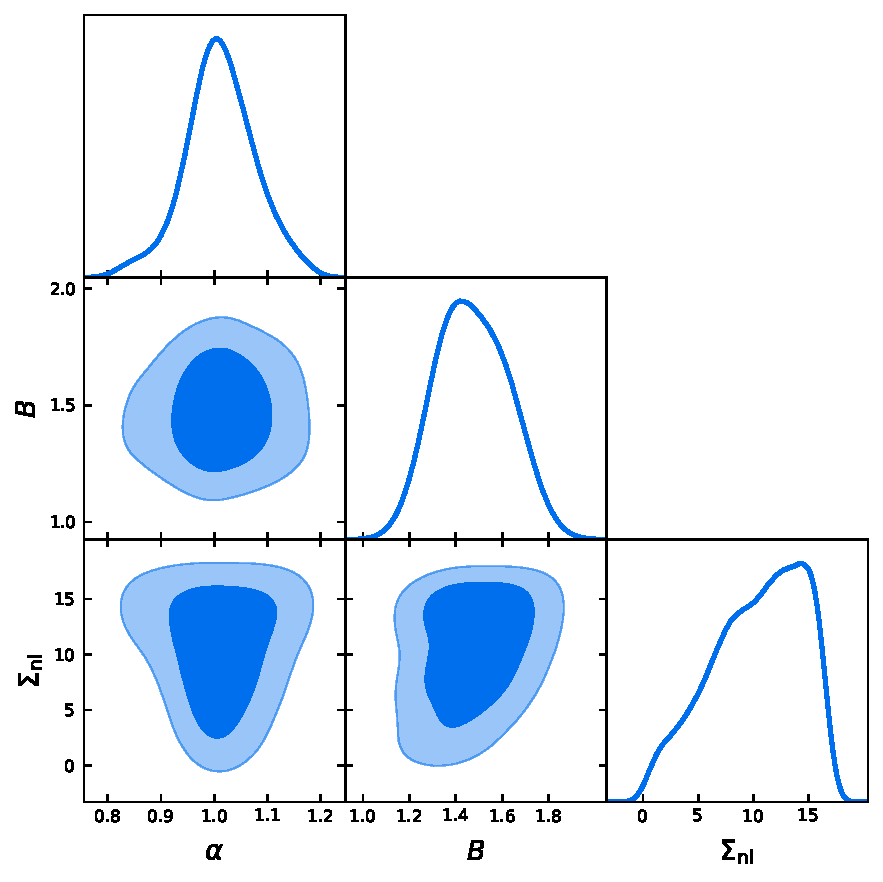
\includegraphics[width=0.9\linewidth]{plots/TwoPCF_mockavg_allsyst_v7_gal_cbz_triplot}
\end{figure}
\end{multicols}
\pagebreak
\begin{multicols}{2}
\begin{figure}
	\centering
	\includegraphics[width=1\linewidth]{plots/{{bestfit_ELG_ALL_bin8_mean_xi0_nosyst.gal}}}
	\caption{$\chi^2_{\mathrm{best}}/$dof$=0.04$ }
\end{figure}
\begin{figure}
	\centering
	\includegraphics[width=1\linewidth]{plots/{{bestfit_ELG_ALL_bin8_mean_xi0_allsyst.gal}}}
	\caption{$\chi^2_{\mathrm{best}}/$dof $=0.06 $}
\end{figure}

\end{multicols}
\end{frame}
\section{Results}
\begin{frame}[allowframebreaks]{Results: Mean 2PCF Voids}
\begin{multicols}{2}
	\textbf{No systematics}
	\begin{figure}
		\centering
		\includegraphics[width=0.9\linewidth]{plots/{{TwoPCF_mockavg_nosyst_v7_void_R-15.5-50_cbz_triplot}}}
	\end{figure}
	\textbf{All systematics}
	\begin{figure}
		\centering
	\includegraphics[width=0.9\linewidth]{plots/{{TwoPCF_mockavg_allsyst_v7_void_R-15.5-50_cbz_triplot}}}
	\end{figure}
\end{multicols}
\pagebreak
\begin{multicols}{2}
\begin{figure}
	\centering
	\includegraphics[width=1\linewidth]{plots/{{bestfit_TwoPCF_mockavg_nosyst_v7_void_R-15.5-50_cbz_nosyst.void}}}
	\caption{$\chi^2_{\mathrm{best}}/$dof$=0.36$}
\end{figure}
\begin{figure}
	\centering
	\includegraphics[width=1\linewidth]{plots/{{bestfit_TwoPCF_mockavg_allsyst_v7_void_R-15.5-50_cbz_allsyst.void}}}
	\caption{$\chi^2_{\mathrm{best}}/$dof$=0.42$ }
\end{figure}
\end{multicols}
\end{frame}
\begin{frame}[allowframebreaks]{Results: Mean2PCF Comparison}
\begin{table}
	\begin{tabular}{ccc}
	&Galaxies&Voids\\
$\alpha_{\mathrm{all}} - \alpha_{\mathrm{none}}$&$\num[scientific-notation=true]{0.00334 \pm 0.00289}$&$\num[scientific-notation=true]{-0.00099 \pm 0.00729}$
	\end{tabular}
\end{table}
 
\begin{figure}
	\centering
	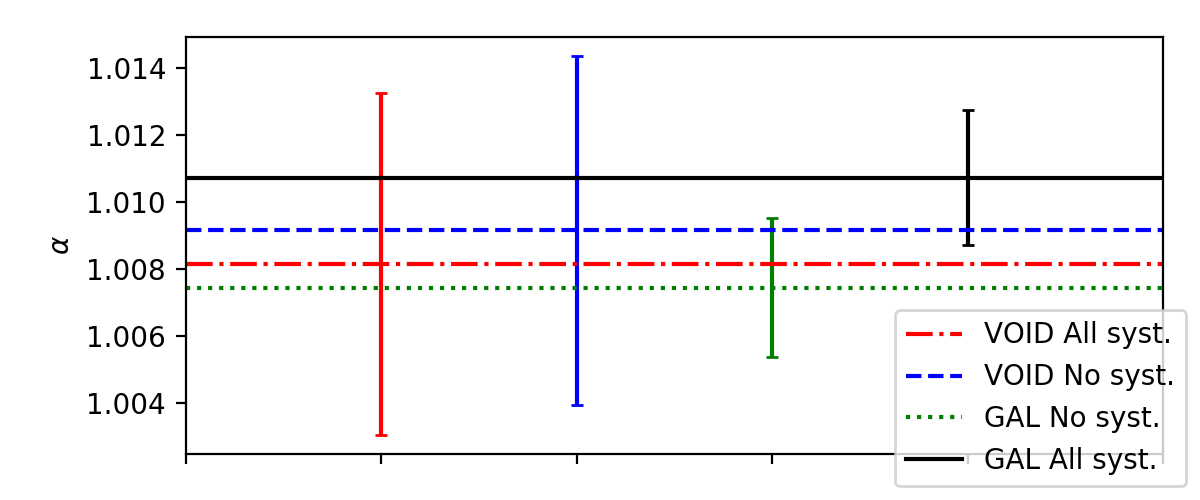
\includegraphics[width=0.7\linewidth]{plots/alpha_mean_comparison_ALLvsNO}
	\caption{Fit results for the dilation parameter $\alpha$ when using the mean of the mocks.}
	\label{fig:alphameancomparisonallvsno}
\end{figure}

\end{frame}
\begin{frame}[allowframebreaks]{Results: Individual 2PCF}
	\begin{table}
		\begin{tabular}{ccc}
			&Galaxies&Voids\\
			$\alpha_{\mathrm{all}} - \alpha_{\mathrm{none}}$&$\num[scientific-notation=true]{0.00189 \pm 0.00239}$&$\num[scientific-notation=true]{-0.00107 \pm 0.00239}$
		\end{tabular}
	\end{table}
	\begin{multicols}{2}
	\begin{figure}
	\centering
	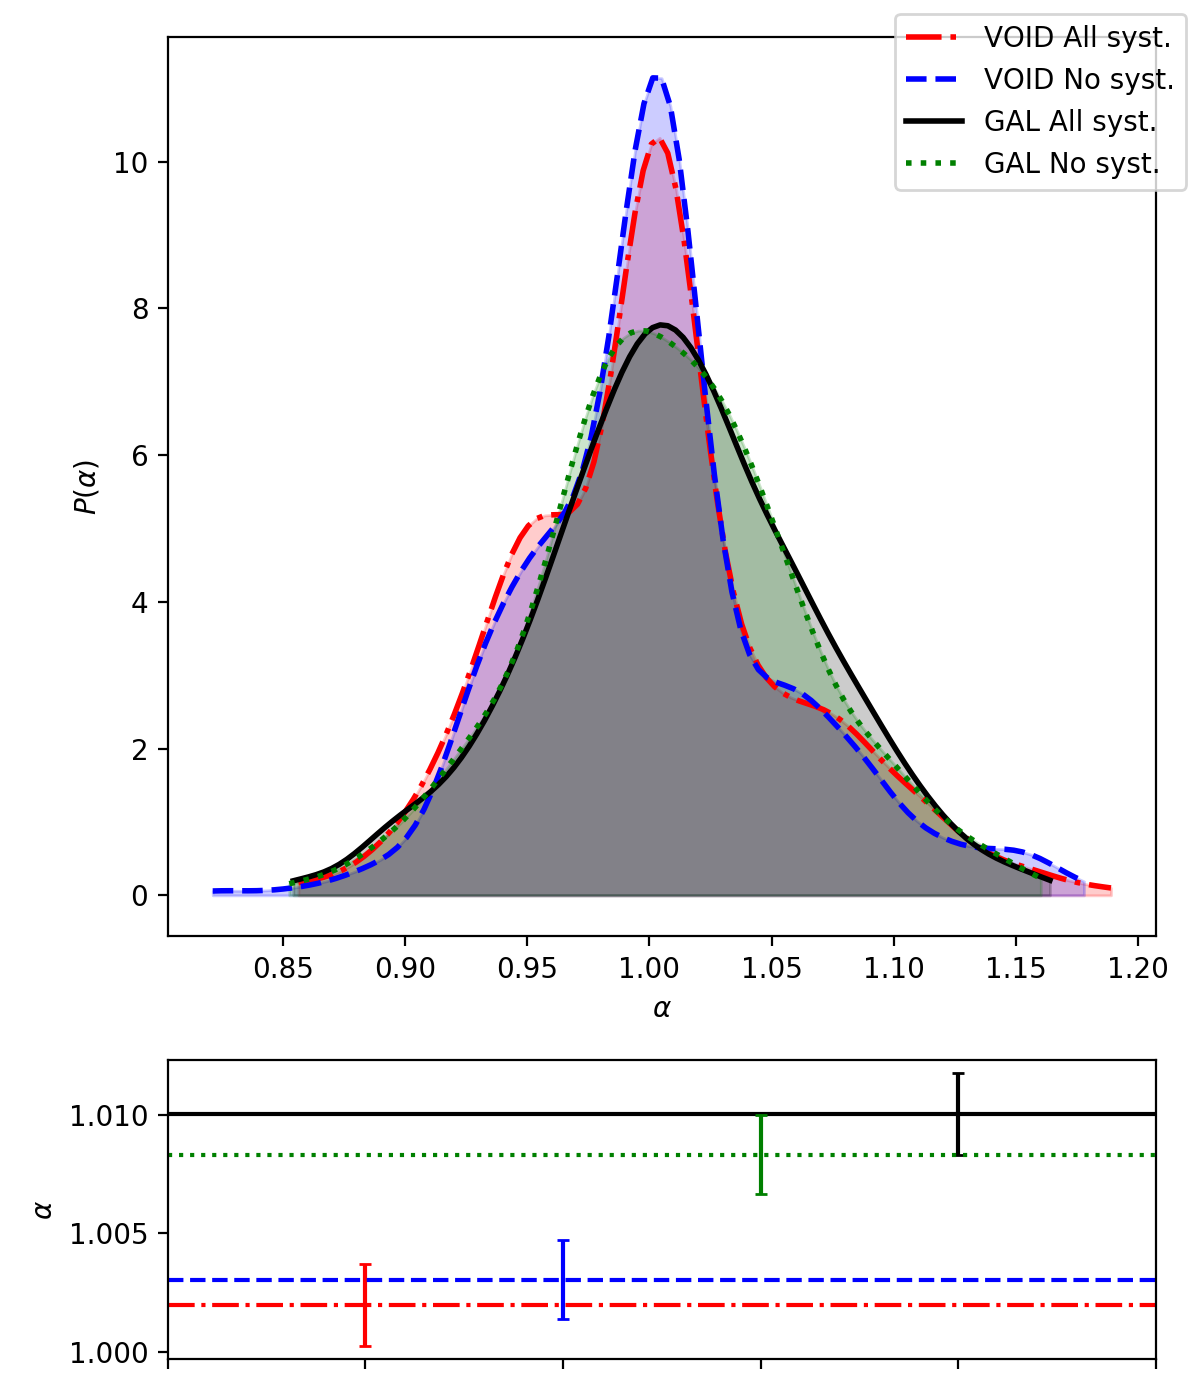
\includegraphics[width=0.8\linewidth]{plots/alpha_comparison_ALLvsNO}
	\caption{Fit results for the $\alpha$ parameter from fitting each of the mocks individually. Top panel shows the distributions obtained. Bottom panel shows the mean values and the (scaled) standard deviation as error.}
	\label{fig:alphacomparisonallvsno}
\end{figure}

	\end{multicols}
\end{frame}
\section{Conclusions}
\begin{frame}[allowframebreaks]{Conclusions}
\begin{itemize}
	\item The fit to the mean 2PCF shows a smaller shift due to systematics in the void case.
	\item The posteriors $p(\alpha|X)$ in the void case have large widths that make it difficult to be confident in the conslusion above.
	\item The individual fits show smaller uncertainty in the void measurement and still show the difference in the peak shift.
	\item Priors can be tweaked to get a better $p(\alpha|X)$ for voids but reduced $\chi^2$ is already close to 1.
	\item Dataset is noisy as shown by the low SNR
	\item The analysis should be repeated with other tracers with better SNR (e.g. LRG)
\end{itemize}
\end{frame}
\appendix
\section<presentation>*{\appendixname}
\subsection<presentation>*{References}

\begin{frame}[allowframebreaks]
  \frametitle<presentation>{References}
    	\printbibliography[heading=bibintoc, title={References}]

\end{frame}

\end{document}


